\subsection{Schéma úpravy modifikátora}
Táto metóda upravuje gradient účelovej funkcie nominálneho modelu na základe odhadnutého gradientu zariadenia, presne ako uvádza rovnica \eqref{eq:mas_chemostat_modifierValue}. Práve s odhadom gradientu môžu nastať komplikácie, najmä kvôli šumu merania. Z tohto dôvodu najskôr demonštrujeme funkčnosť tejto metódy tak, že namiesto odhadnutého gradientu budeme používať skutočný gradient účelovej funkcie zariadenia, teda Monod modelu. 

Ako môžeme vidieť na Obr. \ref{fig:mas_realGrad_costF}, tak takýto prístup dokáže zabezpečiť, že za určitý počet iterácií dosiahneme optimálnu prevádzku zariadenia. Na tomto obrázku sú znázornené priebehy optím upravenej účelovej funkcii, ktoré sú vyjadrené ako hodnoty účelovej funkcie zariadenia, pri rôznych váhových koeficientoch $ c $. Všimnime si, že rýchlosť konvergencie závisí od veľkosti váhového koeficientu $ c $. Ak sa pozrieme na rovnicu \eqref{eq:mas_correction}, vidíme, že čím menšia je hodnota $ c $ tak, tým viac nových informácií o gradiente vkladáme do modifikátora $ \lambda $. Na vedľajšom obrázku \ref{fig:mas_realGrad_lam} sú znázornené príslušné priebehy hodnôt modifikátora v jednotlivých iteráciách. Z tohto obrázka je zrejmé, že ak modifikátor nadobudne hodnotu, ktorá je zobrazená bodkovane a je definovaná rovnicou \eqref{eq:mas_opt_lambda}, dosiahneme optimum zariadenia. Tento fakt možno sledovať aj na Obr. \ref{fig:mas_costFun_compar}, ktorý zobrazuje hodnoty účelových funkcií zariadenia, nominálneho modelu a upravenej účelovej funkcie pri rôznych rýchlostiach riedenia $ D $. Na tomto obrázku môžeme vidieť, že úprava gradientu účelovej funkcie nominálneho modelu, stačí na dosiahnutie optimálnej prevádzky.

\begin{figure}
	\centering
	\begin{subfigure}[b]{0.49\textwidth}
		\centering
		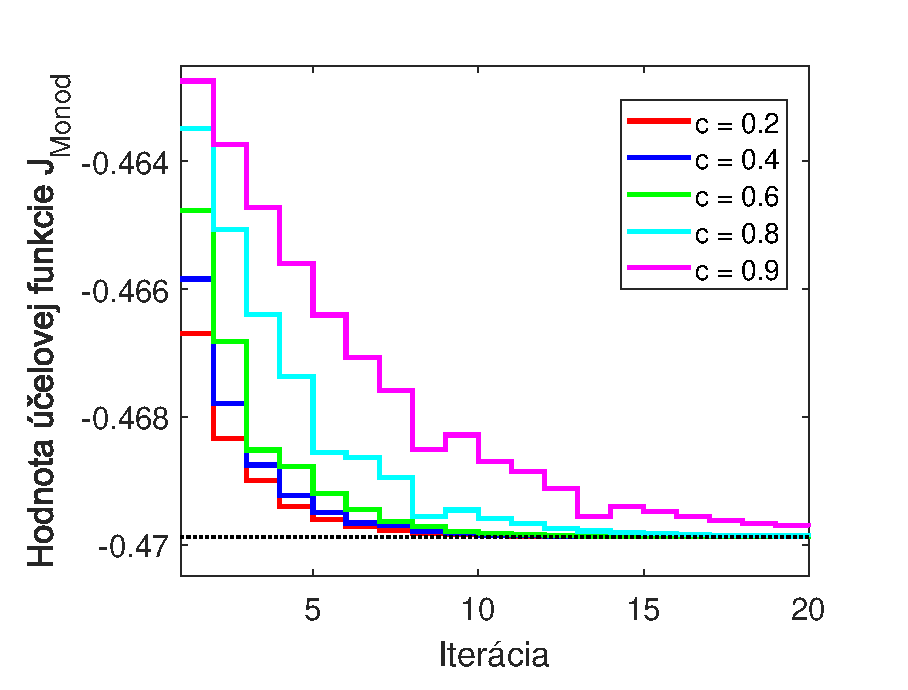
\includegraphics[width=\linewidth]{images/mas_woNoise_costFun}
		\caption{Optimá upravenej účelovej funkcie vyjadrené ako hodnoty účelovej funkcie Monod modelu (zariadenia).}
		\label{fig:mas_realGrad_costF}
	\end{subfigure}
	\hfill
	\begin{subfigure}[b]{0.49\textwidth}
		\centering
		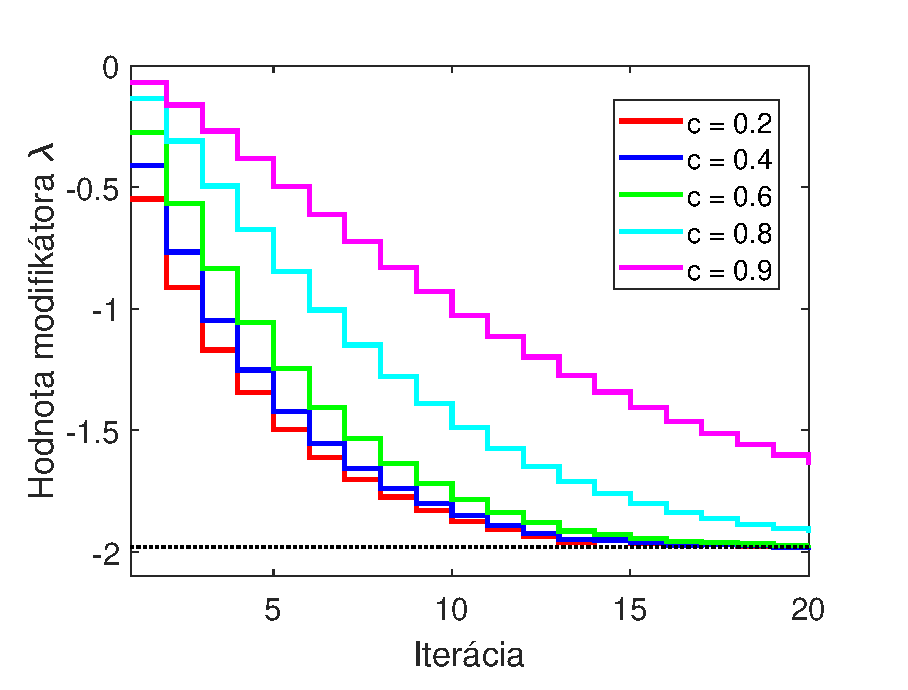
\includegraphics[width=\linewidth]{images/mas_woNoise_lam}
		\caption{Priebeh hodnôt modifikátora. \newline \newline}
		\label{fig:mas_realGrad_lam}
	\end{subfigure}
	\caption{Priebeh schémy úpravy modifikátora s využitím skutočného gradientu účelovej funkcie pri rôznych hodnotách váhových koeficientov $ c $.}
\end{figure}

\begin{figure}
	\centering
	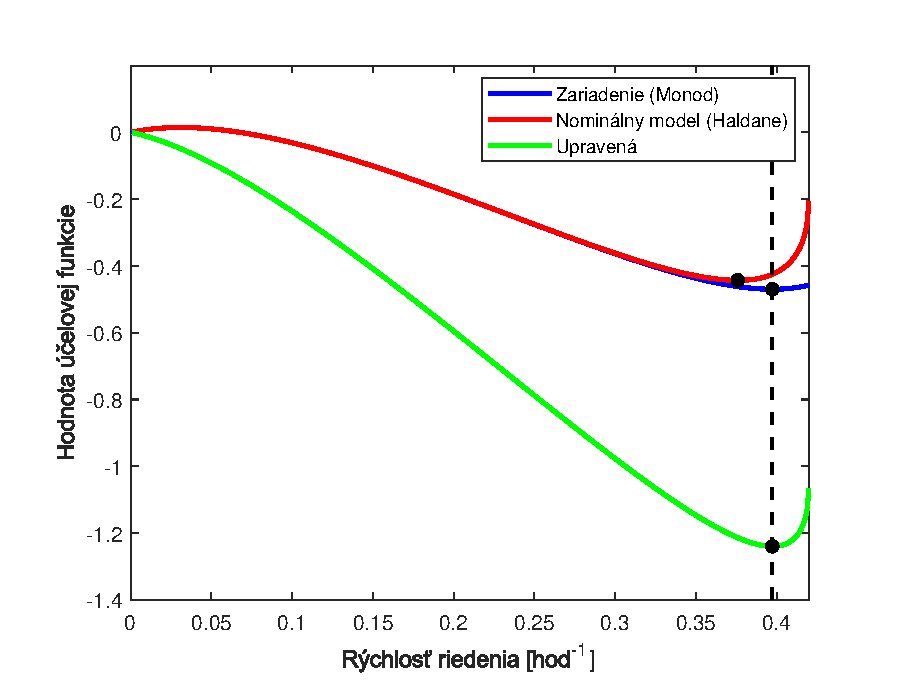
\includegraphics[width=0.7\linewidth]{images/mas_costFun_compar}
	\caption{Porovnanie účelových funkcií a ich optím.}
	\label{fig:mas_costFun_compar}
\end{figure}

Pozrime sa teraz, ako by sa zmenila situácia, ak by sme skutočný gradient vymenili za odhadnutý. Výsledky tejto simulácie môžeme vidieť na Obr. \ref{fig:mas_noiseDist_costF} a \ref{fig:mas_noiseDist_lam}, ktoré zobrazujú, podobne ako v predchádzajúcom prípade, riešenia upravenej optimalizačnej úlohy, vyjadrené ako hodnoty účelovej funkcie Monod modelu a priebeh príslušných hodnôt modifikátora v jednotlivých iteráciách pri rôznej maximálnej hodnote šumu merania $ \left|e\right| $. Ako si môžeme všimnúť, tak vplyv šumu merania je zrejmý a môže pôsobiť dvojako. Na jednej strane môže zabezpečiť rýchlejšiu konvergenciu ako je tomu na Obr.  \ref{fig:mas_noiseDist}. Na druhej strane, ak rozdiel v hodnotách ustálených stavov je porovnateľný alebo menší ako vplyv šumu, vznikajú oscilácie, a tým sa znemožňuje presná konvergencia. Amplitúdu oscilácií môžeme tlmiť zväčšovaním hodnoty váhového koeficientu $ c $, ale to znamená veľmi pomalú konvergenciu. V horšom prípade, ak odhadnutý gradient nadobudne rádovo väčšiu hodnotu od skutočného, pozmení tým aj hodnotu modifikátora, ktorá sa potom bude tiež veľmi pomaly vracať späť na pôvodnú hodnotu. Samozrejme, stále je tu hrozba, že vplyv šumu môže viesť k takým hodnotám modifikátora, ktoré dostanú náš systém do nežiaduceho stavu napr. do výplachu. 
\begin{figure}
	\centering
	\begin{subfigure}[b]{0.49\textwidth}
		\centering
		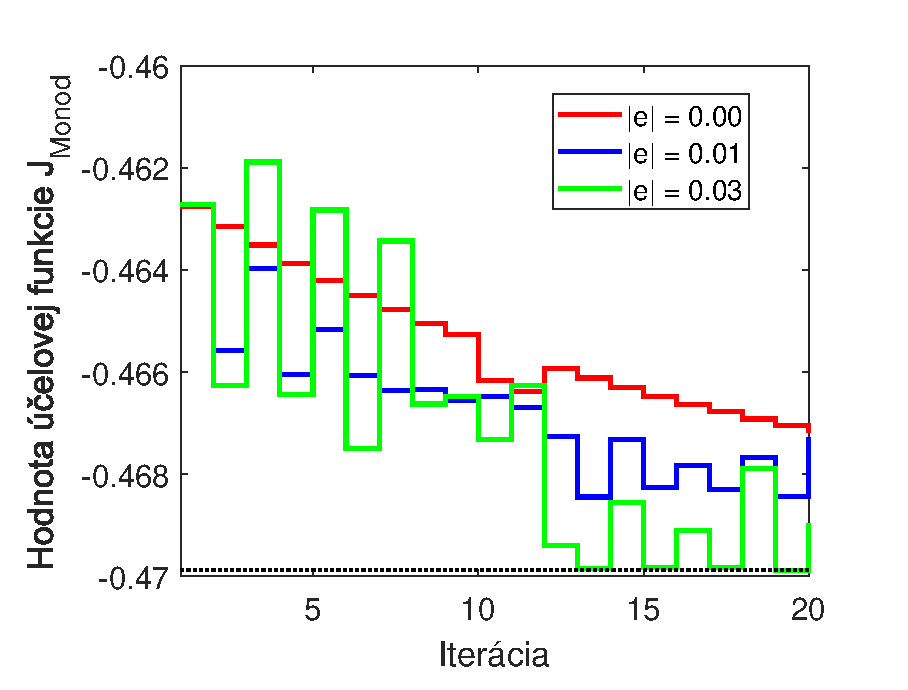
\includegraphics[width=\linewidth]{images/mas_noiseDist_costFun}
		\caption{Optimá upravenej účelovej funkcie vyjadrené ako hodnoty účelovej funkcie Monod modelu (zariadenia).}
		\label{fig:mas_noiseDist_costF}
	\end{subfigure}
	\hfill
	\begin{subfigure}[b]{0.49\textwidth}
		\centering
		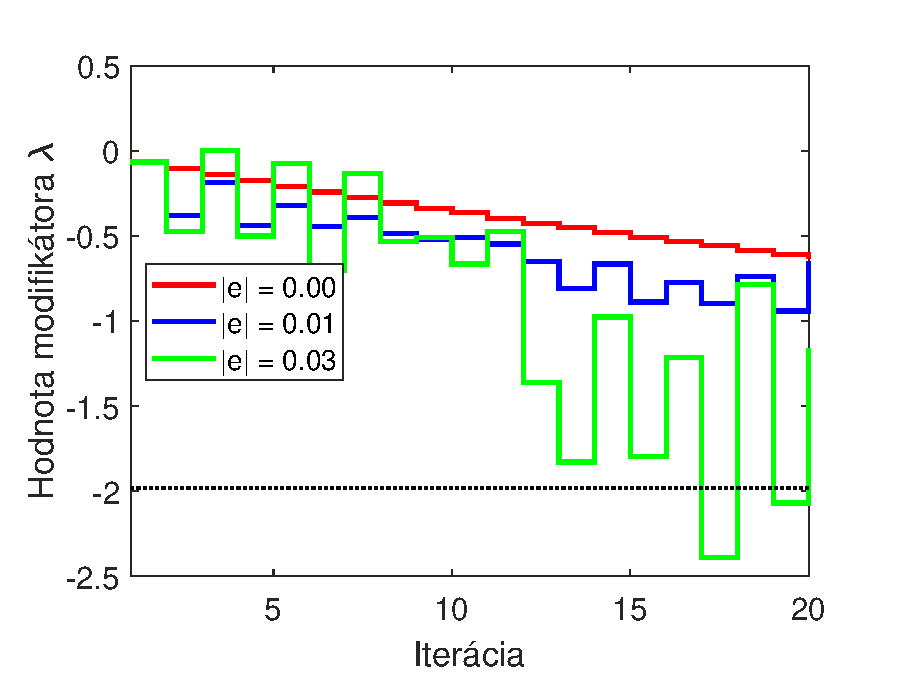
\includegraphics[width=\linewidth]{images/mas_noiseDist_lam}
		\caption{Priebeh hodnôt modifikátora. \newline \newline}
		\label{fig:mas_noiseDist_lam}
	\end{subfigure}
	\caption{Priebeh schémy úpravy modifikátora s využitím odhadu gradientu účelovej funkcie pri rôznom rozptyle šumu merania $ \left|e\right| $ a hodnote váhového koeficientu $ c = 0.945 $.}
	\label{fig:mas_noiseDist}
\end{figure}

Mali by sme pripomenúť ešte zopár technických poznámok. Aby sme rozbehli túto metódu optimalizácie prevádzky zariadenia, potrebujeme mať na začiatku informácie o dvoch skokových zmenách na prvý odhad gradientu resp. výpočet modifikátora. Veľkosť počiatočnej skokovej zmeny je veľmi podstatná, pretože súvisí s počiatočnou hodnotou odhadovaného gradientu a tým ovplyvňuje celkový priebeh optimalizácie, najmä pri vysokých hodnotách váhového koeficientu $ c $. Z tohto dôvodu sme aj my zvolili počiatočnú skokovú zmenu z ustáleného stavu pri $ D = 0.1\si{\per\hour} $ na $ D_{N}^{\star} = 0.376\si{\per\hour} $, aby sme zabezpečili spoľahlivý počiatočný odhad gradientu. Ďalšia pripomienka, ktorá stojí za zváženie, je ohraničenie zmeny odhadu gradientu. Kvôli vplyvu šumu, sa môžu dva po sebe idúce odhadnuté gradienty rádovo líšiť. Dôsledok toho je, že to vedie k osciláciám riešenia s veľkou amplitúdou, v horšom prípade to môže spôsobiť problémy pri riešení optimalizačnej úlohy. 

Ako sme ukázali, tak metóda úpravy účelovej funkcie nominálneho modelu pomocou modifikátora, môže nájsť optimálny ustálený stav zariadenia. Problematickým je vplyv šumu merania, ktorý ak je výraznejší ako samotný rozdiel v skokových zmenách, tak nedokážeme zabezpečiť konvergenciu k optimu. Preto treba vhodne nastaviť parametre tejto metódy, čo vôbec nie je jednoduchá úloha, najmä v prípade biochemického reaktora, kde fluktuácia koncentrácie biomasy je značná.
